% fig_pott_timing.tex
% TR-33: Horizontal timeline comparing POTT vs conventional Zone 2 trip
%
% Timeline: 0 ms to 350 ms
% Key events:
%   0 ms      : fault inception
%  20 ms      : Zone 1 trips (alpha <= 0.80) — blue
%  30 ms      : remote 67Q/87L asserts at End B
%  32 ms      : POTT trip at End A (carrier arrives) — green
% 100 ms      : Memory polarisation expires — vertical red dashed
% 300 ms      : Conventional Zone 2 timer fires — but memory already expired → FAIL
%
% Three swim-lanes: Zone 1, POTT path, Conventional Zone 2

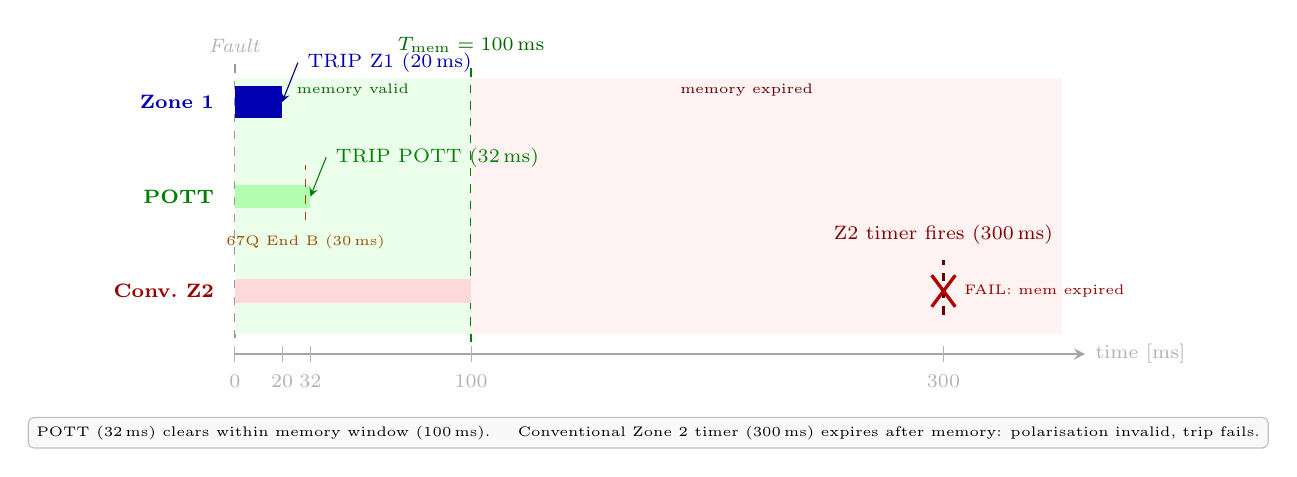
\begin{tikzpicture}[
  every node/.style = {font=\scriptsize},
]

%% ── Scale: 1 cm = 50 ms ──────────────────────────────────────────────────────
\def\sc{0.030}   % 1ms = 0.030cm  →  350ms = 10.5cm

%% ── Derived x-coordinates (hardcoded) ───────────────────────────────────────
% 0ms=0, 20ms=0.60, 30ms=0.90, 32ms=0.96, 100ms=3.00, 300ms=9.00, 350ms=10.50
\def\xO{0}
\def\xZ{0.60}
\def\xRem{0.90}
\def\xPOTT{0.96}
\def\xMem{3.00}
\def\xConv{9.00}
\def\xEnd{10.50}

%% ── Lane y-coordinates ───────────────────────────────────────────────────────
\def\yZ{2.4}     % Zone 1 lane
\def\yP{1.2}     % POTT lane
\def\yC{0.0}     % Conventional Zone 2 lane
\def\yAx{-0.8}  % time axis

%% ── Time axis ────────────────────────────────────────────────────────────────
\draw[->, >=stealth, gray!70, thick]
  (\xO, \yAx) -- (\xEnd+0.3, \yAx)
  node[right, gray!60] {time [ms]};

% Tick marks and labels
\foreach \xms/\lab in {0/0, 0.60/20, 0.96/32, 3.00/100, 9.00/300}{
  \draw[gray!60, thin] (\xms, \yAx-0.10) -- (\xms, \yAx+0.10);
  \node[gray!60, below=4pt] at (\xms, \yAx) {\lab};
}

%% ── Fault inception marker ───────────────────────────────────────────────────
\draw[gray!80, thick, dashed] (\xO, \yAx+0.2) -- (\xO, \yZ+0.5);
\node[gray!60, above] at (\xO, \yZ+0.5) {\textit{Fault}};

%% ── Memory window (green shading, 0 to 100 ms) ───────────────────────────────
\fill[green!8]  (\xO, \yAx+0.25) rectangle (\xMem, \yZ+0.3);
\draw[green!50!black, thick, dashed] (\xMem, \yAx+0.15) -- (\xMem, \yZ+0.5);
\node[green!40!black, above] at (\xMem, \yZ+0.5)
  {$T_\mathrm{mem}=100$\,ms};
\node[green!40!black, font=\tiny] at (1.5, \yZ+0.15)
  {memory valid};

%% ── Post-memory shading ──────────────────────────────────────────────────────
\fill[red!5] (\xMem, \yAx+0.25) rectangle (\xEnd, \yZ+0.3);
\node[red!40!black, font=\tiny] at (6.5, \yZ+0.15)
  {memory expired};

%% ── Lane labels ──────────────────────────────────────────────────────────────
\node[font=\scriptsize\bfseries, blue!70!black, left=4pt]
  at (\xO, \yZ) {Zone~1};
\node[font=\scriptsize\bfseries, green!50!black, left=4pt]
  at (\xO, \yP) {POTT};
\node[font=\scriptsize\bfseries, red!60!black, left=4pt]
  at (\xO, \yC) {Conv.\ Z2};

%% ── Zone 1 trip bar (0 to 20 ms) ─────────────────────────────────────────────
\fill[blue!70!black] (\xO, \yZ-0.20) rectangle (\xZ, \yZ+0.20);
\draw[blue!50!black, <-, >=stealth]
  (\xZ, \yZ) -- (\xZ+0.2, \yZ+0.5)
  node[right, blue!70!black] {TRIP Z1 (20\,ms)};

%% ── POTT path ────────────────────────────────────────────────────────────────
% Waveform: Zone 2 assert bar (instant) then wait for carrier
\fill[green!30] (\xO, \yP-0.15) rectangle (\xPOTT, \yP+0.15);
\draw[green!50!black, <-, >=stealth]
  (\xPOTT, \yP) -- (\xPOTT+0.2, \yP+0.5)
  node[right, green!50!black] {TRIP POTT (32\,ms)};

% Remote 67 assertion marker
\draw[orange!60!black, thin, dashed]
  (\xRem, \yP-0.3) -- (\xRem, \yP+0.4);
\node[orange!60!black, font=\tiny, below=2pt] at (\xRem, \yP-0.3)
  {67Q End B (30\,ms)};

%% ── Conventional Zone 2 path ─────────────────────────────────────────────────
% Pre-memory: pending (hatched-ish via fill)
\fill[red!15] (\xO, \yC-0.15) rectangle (\xMem, \yC+0.15);
% Post-memory: faded/expired
\fill[red!5]  (\xMem, \yC-0.15) rectangle (\xConv, \yC+0.15);
\draw[red!40!black, thick, dashed]
  (\xConv, \yC-0.3) -- (\xConv, \yC+0.4);
\node[red!50!black, above=2pt] at (\xConv, \yC+0.4)
  {Z2 timer fires (300\,ms)};
% Cross — trip BLOCKED
\draw[red!70!black, very thick]
  (\xConv-0.15, \yC-0.20) -- (\xConv+0.15, \yC+0.20);
\draw[red!70!black, very thick]
  (\xConv-0.15, \yC+0.20) -- (\xConv+0.15, \yC-0.20);
\node[red!60!black, font=\tiny, right=4pt] at (\xConv, \yC)
  {FAIL: mem expired};

%% ── Caption box ──────────────────────────────────────────────────────────────
\node[draw=gray!50, fill=gray!5, rounded corners=2pt,
      font=\tiny, inner sep=3pt, align=center]
  at (5.25, -1.8)
  {POTT (32\,ms) clears within memory window (100\,ms). \quad
   Conventional Zone~2 timer (300\,ms) expires after memory: polarisation invalid, trip fails.};

\end{tikzpicture}
